\section{Artifact and Reproduction}
The aggregate v0.6 release combines the frozen v0.2 controlled/provenance
surface, prospective robustness extensions, the separately frozen v0.3
external order-book surface, and the frozen v0.6 actual-model proposal
extension. Every data and result layer records a configuration hash, data hash,
split registry, seed registry, output hashes, and claim boundary. The aggregate
verifier transitively checks the earlier surfaces and the v0.6 freeze-to-result
chain; the repository suite is rerun before release. The controlled paper
test is bound to content-addressed archive \texttt{be95f4d1...98aa8} and took
80.59 seconds on the development machine with peak resident memory about
550 MB. Re-running any inspected one-time paper test is prohibited except for a
versioned correctness defect that preserves the original output.

\begin{table*}[h]
  \caption{\textbf{FinAuth-Audit treats benchmark validity as the evaluation object.} ``Rules'' denotes explicit comparison of execution or decision rules; the remaining columns denote validity audits, not generic safety features.}
  \label{tab:benchmark_comparison}
  \centering
  \benchmarktableformat
  % Generated by finauth_audit/paper/generate_tables.py. Do not edit manually.
\begin{tabular}{llcccc}
\toprule
Benchmark & Evaluation unit & Rules & Coverage audit & Provenance & Power gate \\
\midrule
FinQA~\cite{chen2021finqa} & financial QA & no & no & no & no \\
PIXIU~\cite{xie2023pixiu} & financial tasks & no & no & no & no \\
FinBen~\cite{xie2024finben} & financial tasks & no & no & no & no \\
AgentBench~\cite{liu2023agentbench} & agent tasks & no & no & no & no \\
WebArena~\cite{zhou2023webarena} & web tasks & no & no & no & no \\
Weak experiments~\cite{chou2025weakrules} & experiment portfolios & yes & no & no & no \\
\textbf{FinAuth-Audit} & weak financial priors & yes & yes & yes & yes \\
\bottomrule
\end{tabular}

\end{table*}

\begin{table*}[h]
  \caption{Artifact components and machine-checkable release paths.}
  \label{tab:artifact_checklist}
  \centering
  \benchmarktableformat
  % Generated by finauth_audit/paper/generate_tables.py. Do not edit manually.
\begin{tabular}{p{0.20\linewidth}p{0.35\linewidth}p{0.31\linewidth}}
\toprule
Artifact & Release path & Verification \\
\midrule
Paper test & \path{results/paper_test/} & one-time registry; 5k clusters \\
Community hidden & \path{sealed/community_hidden/} & 5k clusters; unevaluated \\
Freeze archive & \path{manifests/paper_test_snapshots/} & content-addressed SHA-256 \\
Point-in-time layer & \path{results/public_audit/} & power and timestamp gates \\
External order book & \path{results/external_orderbook_v03/} & powered mixed result; 550 checks \\
Actual-model paper test & \path{results/real_agent_v06/paper_test/} & 3 models; 200-date, 2-task aggregate test \\
Historical-memory audit & \path{results/real_agent_v06/historical_memory_audit/} & outcome-blind aggregates; no rationale text persisted \\
Training robustness & \path{results/training_robustness_v03/} & 144 fits; 6 mechanisms \\
Figures & \path{paper/figures/} & PDF, SVG, PNG; text QA \\
HTML and cards & \path{paper/html/}; \path{docs/} & combined paper/supplement; local assets \\
Release archive & \path{dist/finauth-audit-0.6.0.tar.gz} & allowlist; clean-room hash and split scan \\
Verifier & \path{verify_artifact.py} & all frozen surfaces, fields, hashes, and tests \\
\bottomrule
\end{tabular}

\end{table*}

The figure generator writes PDF, SVG, and PNG from one source and records a minimum visible font size of 8 pt. Generation fails if marked point labels overlap. The table generator reads frozen result files and records input/output hashes in \texttt{table\_manifest.json}; no reported numeric result is hand-entered into the manuscript. A page-faithful HTML bundle mirrors the combined PDF, while the benchmark card, reproduction guide, maintenance policy, and external-submission protocol state the community-use contract.

\begin{figure*}[h]
  \centering
  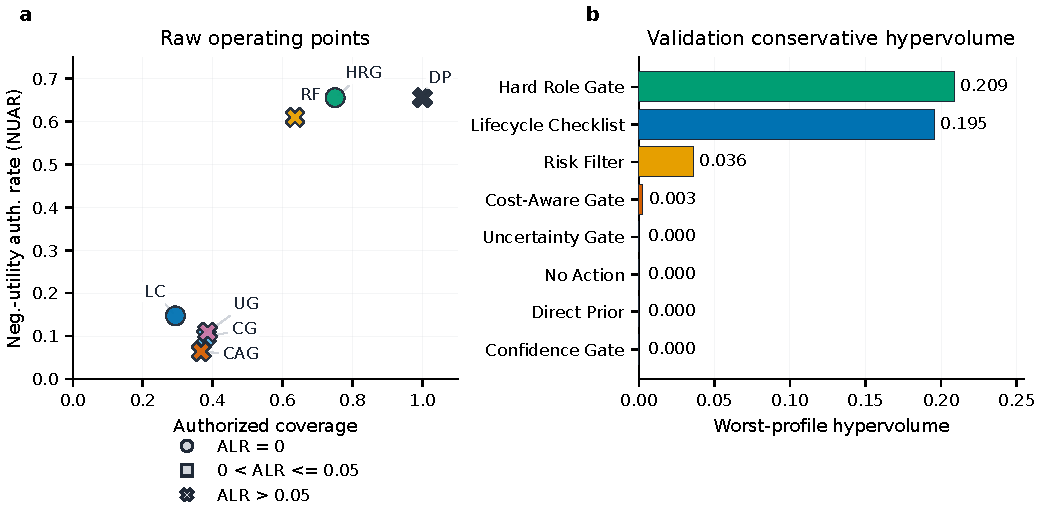
\includegraphics[width=\textwidth]{figures/fig_certification_surface.pdf}
  \Description{Two-panel validity figure. The left panel plots paper-test rule coverage against negative-utility authorization rate with marker shape indicating authority-laundering strata. The right panel ranks validation worst-profile conservative hypervolume.}
  \caption{\textbf{NUAR, lineage integrity, coverage, and conservative hypervolume produce different rule orderings.} Panel (a) reports one-time paper-test operating points; marker shape encodes ALR strata. Short labels are DP (Direct Prior), CG (Confidence Gate), UG (Uncertainty Gate), RF (Risk Filter), CAG (Cost-Aware Gate), HRG (Hard Role Gate), and LC (Lifecycle Checklist). Panel (b) is a pre-frozen validation sensitivity, not a second paper-test ranking. Zero authorization produces NUAR and ALR \textit{N/A}, not zero.}
  \label{fig:certification}
\end{figure*}

\section{Controlled Certification Details}
The controlled evaluation excludes the explicit no-opportunity slice from certification but reports it as a negative control. Table~\ref{tab:certification_profiles} gives the cluster-bootstrap bounds used by the frozen 120-cell surface. A zero-action bootstrap replicate contributes coverage zero and execution-denominator metrics \textit{N/A}. If every replicate is undefined, no dependent cell passes.

\begin{table*}[h]
  \caption{\textbf{Pre-frozen policy families and continuous hypervolume do not define a universal winner.} Values are worst-profile validation pass fractions over each author-specified grid. The conservative family certifies no rule; Lifecycle has nonzero balanced and coverage-first volume, while Hard Role Gate has the largest continuous conservative hypervolume. These are sensitivity diagnostics, not practitioner-elicited thresholds.}
  \label{tab:policy_families}
  \centering
  \benchmarktableformat
  % Generated by finauth_audit/paper/generate_tables.py. Do not edit manually.
\begin{tabular}{lrrrr}
\toprule
Rule & Conservative & Balanced & Coverage-first & Continuous HV \\
\midrule
No Action & 0.000 & 0.000 & 0.000 & 0.000 \\
Direct Prior & 0.000 & 0.000 & 0.000 & 0.000 \\
Confidence Gate & 0.000 & 0.000 & 0.000 & 0.000 \\
Uncertainty Gate & 0.000 & 0.000 & 0.000 & 0.000 \\
Risk Filter & 0.000 & 0.000 & 0.000 & 0.036 \\
Cost-Aware Gate & 0.000 & 0.000 & 0.000 & 0.003 \\
Hard Role Gate & 0.000 & 0.000 & 0.000 & 0.209 \\
Lifecycle Checklist & 0.000 & 0.375 & 0.188 & 0.195 \\
\bottomrule
\end{tabular}

\end{table*}

\begin{table*}[h]
\caption{One-sided cluster-bootstrap bounds and certification volumes by rule and profile on the paper test.}
  \label{tab:certification_profiles}
  \centering
  \benchmarktableformat
  % Generated by finauth_audit/paper/generate_tables.py. Do not edit manually.
\begin{tabular}{llrrrr}
\toprule
Rule & Profile & Coverage LCB & NUAR UCB & ALR UCB & Cert. volume \\
\midrule
No Action & overall & 0.000 & \textit{N/A} & \textit{N/A} & 0.000 \\
No Action & stress & 0.000 & \textit{N/A} & \textit{N/A} & 0.000 \\
Direct Prior & overall & 1.000 & 0.667 & 0.250 & 0.000 \\
Direct Prior & stress & 1.000 & 0.712 & 0.250 & 0.000 \\
Confidence Gate & overall & 0.370 & 0.107 & 0.253 & 0.000 \\
Confidence Gate & stress & 0.341 & 0.161 & 0.254 & 0.000 \\
Uncertainty Gate & overall & 0.375 & 0.117 & 0.250 & 0.000 \\
Uncertainty Gate & stress & 0.346 & 0.174 & 0.250 & 0.000 \\
Risk Filter & overall & 0.625 & 0.624 & 0.211 & 0.000 \\
Risk Filter & stress & 0.469 & 0.678 & 0.177 & 0.000 \\
Cost-Aware Gate & overall & 0.356 & 0.069 & 0.247 & 0.000 \\
Cost-Aware Gate & stress & 0.302 & 0.053 & 0.248 & 0.000 \\
Hard Role Gate & overall & 0.750 & 0.667 & 0.000 & 0.000 \\
Hard Role Gate & stress & 0.750 & 0.713 & 0.000 & 0.000 \\
Lifecycle Checklist & overall & 0.285 & 0.156 & 0.000 & 0.300 \\
Lifecycle Checklist & stress & 0.233 & 0.127 & 0.000 & 0.400 \\
\bottomrule
\end{tabular}

\end{table*}

The paper-test opportunity rates are ordinary 0.450, moderate stress 0.386, severe stress 0.236, rare safe opportunity 0.131, high missed opportunity 0.507, stress-only period 0.195, and no-opportunity control 0.000. The oracle-positive label is outcome-only and is never available to a rule.

\section{Provenance Definitions and Strata}
Direct leakage authorizes a currently ineligible source. Indirect leakage authorizes a currently eligible source whose original authority is ineligible. ALR uses the same authorized-action denominator as indirect laundering truth. Safe-delegation coverage is the fraction of eligible delegated positive opportunities that remain authorized; false block is its complement. Table~\ref{tab:provenance_traceability} separates the traceable and untraceable strata.

\begin{table*}[h]
\caption{Traceability-specific provenance outcomes on the paper test. \textit{N/A} is structural when a rule authorizes zero rows in a stratum.}
  \label{tab:provenance_traceability}
  \centering
  \benchmarktableformat
  % Generated by finauth_audit/paper/generate_tables.py. Do not edit manually.
\begin{tabular}{llrrrl}
\toprule
Rule & Traceability & Cov. & ALR & Safe del. & False block \\
\midrule
EPV Adapter & traceable & 0.288 & 0.148 & 0.999 & 0.001 \\
EPV Adapter & untraceable & 0.338 & 0.248 & 0.998 & 0.002 \\
Hard Role Gate & traceable & 0.851 & 0.150 & 1.000 & 0.000 \\
Hard Role Gate & untraceable & 1.000 & 0.254 & 1.000 & 0.000 \\
Lifecycle Checklist & traceable & 0.325 & 0.145 & 0.999 & 0.001 \\
Lifecycle Checklist & untraceable & 0.378 & 0.244 & 0.998 & 0.002 \\
No Action & traceable & 0.000 & \textit{N/A} & 0.000 & 1.000 \\
No Action & untraceable & 0.000 & \textit{N/A} & 0.000 & 1.000 \\
No Role Gate & traceable & 1.000 & 0.249 & 1.000 & 0.000 \\
No Role Gate & untraceable & 1.000 & 0.254 & 1.000 & 0.000 \\
Provenance Hard Gate & traceable & 0.724 & 0.000 & 1.000 & 0.000 \\
Provenance Hard Gate & untraceable & 0.000 & \textit{N/A} & 0.000 & 1.000 \\
Provenance Learned Gate & traceable & 0.627 & 0.015 & 0.676 & 0.324 \\
Provenance Learned Gate & untraceable & 0.497 & 0.035 & 0.668 & 0.332 \\
Shared Threshold & traceable & 0.370 & 0.249 & 1.000 & 0.000 \\
Shared Threshold & untraceable & 0.376 & 0.252 & 0.999 & 0.001 \\
Soft Penalty & traceable & 0.404 & 0.234 & 1.000 & 0.000 \\
Soft Penalty & untraceable & 0.416 & 0.254 & 0.999 & 0.001 \\
\bottomrule
\end{tabular}

\end{table*}

Traceable rows include the attested lineage-role chain needed to detect laundering in principle. Untraceable rows omit that evidence. On the paper test, Provenance Hard Gate has traceable coverage 0.724 and untraceable coverage zero; its untraceable NUAR and ALR are undefined rather than zero. The empirical current-role-only Bayes error lower bound rises from 0.129 on traceable rows to 0.256 on untraceable rows, while legal partial signatures reduce the corresponding bounds to 0.061 and 0.083. This is an evidence-availability boundary, not a claim that a detector should infer hidden lineage.

\paragraph{Proof of Equation~\eqref{eq:provenance-bayes-risk}.}
For a fixed observable signature $x$, any deterministic rule $h$ predicts either zero or one. Its error mass at $x$ is therefore either $\Pr(X=x,L=1)$ or $\Pr(X=x,L=0)$, and the smaller achievable mass is their minimum. Summing independently over signatures proves the first equality. A randomized rule takes a convex combination of the same two error masses and cannot improve the minimum. Under equal priors, write $p_\ell(x)=\Pr(X=x\mid L=\ell)$; then
\begin{align*}
 \sum_x \min\{\tfrac12p_0(x),\tfrac12p_1(x)\}
 &=\tfrac12\left(1-\tfrac12\sum_x|p_0(x)-p_1(x)|\right)\\
 &=\tfrac12(1-\mathrm{TV}(P_0,P_1)).
\end{align*}
The audit uses empirical signature frequencies in place of joint probabilities. Its minority count is the exact minimum empirical error for rules using that signature, not a distribution-free bound for another institution or period.

\paragraph{Derivation of Equation~\eqref{eq:provenance-partial-id}.}
Write $q(x)=\Pr(L=1\mid X=x)$. For any rule with positive coverage,
$\mathrm{ALR}(a)=\mathbb{E}[a(X)q(X)]/\mathbb{E}[a(X)]$.
Multiplying the pointwise bounds $\ell(x)\le q(x)\le u(x)$ by the
nonnegative weight $a(x)\Pr(X=x)$, summing, and dividing by coverage gives
Equation~\eqref{eq:provenance-partial-id}. Pointwise-compatible choices of
$q(x)$ attain both endpoints. If resolved signatures have $u=\ell$ and
unresolved signatures have $[\ell,u]=[0,1]$, the interval width is exactly
the rule's authorized unresolved mass divided by its total authorized mass.

\begin{table*}[h]
  \caption{\textbf{Legal observability controls the minimum empirical laundering-classification error.} Joint separation is the weighted empirical separation term in Equation~\eqref{eq:provenance-bayes-risk}; the implementation verifies the corresponding overlap identity to numerical precision.}
  \label{tab:provenance_identifiability}
  \centering
  \benchmarktableformat
  % Generated by finauth_audit/paper/generate_tables.py. Do not edit manually.
\begin{tabular}{llrrrr}
\toprule
Traceability & Observable signature & Rows & Collision frac. & Bayes risk & Joint sep. \\
\midrule
traceable & current role only & 32,857 & 1.000 & 0.129 & 0.742 \\
traceable & legal partial signature & 32,857 & 0.720 & 0.061 & 0.877 \\
untraceable & current role only & 7,143 & 1.000 & 0.256 & 0.488 \\
untraceable & legal partial signature & 7,143 & 0.519 & 0.083 & 0.834 \\
\bottomrule
\end{tabular}

\end{table*}

\section{Public Point-in-Time Gate}
The Polymarket metadata window is 2022-01-01 through 2026-07-17. Monthly sampling caps each month at 120 clusters and each series/month at 12 clusters. Twenty-three high-activity months reached the frozen pagination limit and are disclosed as truncated. Historical probability comes from CLOB price history when available and documented public trades otherwise. The fixed decision time is 35\% of scheduled lifecycle; the source probability precedes the decision, and the first execution observation follows it but precedes resolution.

\begin{table*}[h]
  \caption{Public-source classifications and the pre-result power gate. The point-in-time layer remains \texttt{exploratory\_only} because power is below the frozen requirement; no public test outcome is reported.}
  \label{tab:public_power}
  \centering
  \benchmarktableformat
  % Generated by finauth_audit/paper/generate_tables.py. Do not edit manually.
\begin{tabular}{llrrrp{0.29\linewidth}}
\toprule
Layer / source & Clusters & Power & LCB95 & Req. & Classification \\
\midrule
Public point-in-time & 500 (structural) & 0.164 & 0.160 & 0.80 & exploratory\_only \\
polymarket &  &  &  &  & descriptive public-derived \\
polymarket\_repeated &  &  &  &  & excluded from inference \\
gdelt &  &  &  &  & controlled information-shock \\
fred &  &  &  &  & exploratory non-vintage \\
polymarket\_point\_in\_time &  &  &  &  & confirmatory candidate; structural only \\
\bottomrule
\end{tabular}

\end{table*}

The first CLOB-only design produced sufficient histories for 516 candidate markets. A documented read-only trades fallback increased structural usability without creating synthetic probabilities, spread, or depth. An earlier 3,000-cluster design covered only about 19 hours and was rejected as externally narrow before result inspection. Both negative design iterations remain in the project log.

\section{External Order-Book Replication}
The separately versioned v0.3 extension freezes public Binance USD-M futures
banded depth plus one-minute bars and licensed Databento MES BBO before outcome
evaluation. It is observed market-outcome replay with constructed priors and
assigned roles. Binance uses 500 UTC-date paper-test clusters; planning power
under the frozen v0.2 variance model is 0.970 and 0.965 for the two registered
SESOIs. MES uses 140 RTH-session clusters
and is classified as descriptive because its corresponding design powers are
0.528 and 0.514. Feature rows and sealed execution inputs are separate; returns,
post-cost utility, harm, and burden are materialized only after freeze
verification inside the write-once evaluator.

\begin{table*}[h]
  \caption{\textbf{The external intersection-union claim fails, and observed market data do not make weak priors or authority roles observational.} Panel A reports Cost-Aware Gate minus Lifecycle Checklist. Binance is confirmatory; MES is licensed descriptive evidence, and its fixed six-prior laundering contrast is structural. Panel B separates observed, pre-decision derived, benchmark-assigned, and sealed outcome-only fields.}
  \label{tab:external_orderbook}
  \label{tab:external_field_origins}
  \centering
  \benchmarktableformat
  \textit{Panel A: frozen external replication outcomes.}\par\smallskip
  % Generated by finauth_audit/paper/generate_tables.py. Do not edit manually.
\begin{tabular}{llrlrrrp{0.18\linewidth}}
\toprule
Source & Evidence & Clusters & Endpoint & Diff. & 95\% CI & SESOI & Status \\
\midrule
Binance & powered public & 500 & False-auth. burden & -0.017 & [-0.020, -0.014] & $\leq -0.015$ & pass \\
Binance & powered public & 500 & Laundering burden & +0.015 & [+0.014, +0.017] & $\geq +0.020$ & fail \\
Binance & powered public & 500 & Intersection-union & -- & -- & both arms & \textbf{FAIL (1/2)} \\
MES & licensed descriptive & 140 & False-auth. burden & -0.019 & [-0.029, -0.010] & $\leq -0.015$ & descriptive \\
MES & licensed descriptive & 140 & Laundering burden & 1/6 by design & -- & not applied & not an estimand \\
\bottomrule
\end{tabular}

  \par\medskip
  \textit{Panel B: field origins and evaluation boundary.}\par\smallskip
  % Generated by finauth_audit/paper/generate_tables.py. Do not edit manually.
\begin{tabular}{p{0.19\linewidth}p{0.34\linewidth}p{0.39\linewidth}}
\toprule
Origin & Fields & Evaluation boundary \\
\midrule
Observed source & quotes, bars, depth, timestamps & available at or before the registered decision time \\
Pre-decision derived & momentum, volatility, imbalance, spread/cost proxies & deterministic functions of observed source fields \\
Benchmark assigned & prior family, action, confidence, source role, eligibility & frozen weak-prior construction; not observed agent behavior \\
Outcome only & entry/exit prices, return, utility, harm, burden & sealed until the one-time evaluator; illegal for deployable rules \\
\bottomrule
\end{tabular}

  \par\medskip
  \begin{minipage}{0.96\textwidth}
  \small
  \textit{Sensitivity and release boundary.}
  The Binance seven-day moving-block sensitivity preserves the arm-level
  interpretation. At the frozen primary 8-bps fee, only the registered
  \texttt{false\_authorization\_burden} endpoint (negative-utility burden)
  passes. A 4-bps sensitivity passes both arms, whereas 12 bps passes
  neither; these fee-grid results use fewer bootstrap replicates and remain
  secondary. No sensitivity replaces the registered primary. Binance releases
  source archives, official checksums, derived rows, manifests, and code. MES
  reproduction requires Databento entitlement, and row-level licensed data are
  not redistributed. MES is an optional licensed replication layer; all
  headline benchmark functionality and primary controlled/provenance
  evaluations are reproducible without redistributing MES records. The public
  dataset entry, exact schema, date/session definitions, reconstruction scripts,
  manifests, and checksums are documented in the artifact.
  \end{minipage}
\end{table*}

\FloatBarrier

\section{Actual Model Proposal Extension}
The v0.6 extension evaluates actual cached proposal outputs rather than
deterministic agent stubs. GPT-5.4-mini, GPT-5.5, and Claude Sonnet 4.6 receive
the same legal pre-decision context on 300 independent dates assigned across
BTC, ETH, BNB, SOL, and XRP. Each date includes a directional-execution task and
a 25\% risk-limit-increase task. Directional sources are eligible edge
proposers; risk-limit source role is assigned by frozen event-ID parity as an
eligible proposer or evidence-only critic before generation. The chronological
partition is 50 development, 200 one-time paper test, and 50 author-unevaluated
holdout dates. The holdout contexts were sent to the same model configurations
before outcome evaluation; 300 proposal rows were encrypted, their key remains
outside the repository, and the ciphertext was not decrypted.

The development/paper cache contains 1,500 plaintext proposal rows and has raw
schema validity 0.994. Nine expected records remain malformed placeholders,
there are zero repairs, and no outcome-conditioned or favorable rerun is
permitted. One extra record was ignored under the preapproved duplicate/extra
record policy. Rationales and self-reported evidence are retained in private
audit caches but prohibited from every execution rule and excluded from the
aggregate public release. The explicit historical-memory lexical audit finds no
registered retrospective phrase, but cannot establish absence of implicit
model memory.

\begin{table*}[h]
  \caption{\textbf{Economic loss, material harm, and authority violation are distinct zero-shot endpoints.} The table reports overall operating points across \RealAgentRankIndependentUnitCount{} UTC-date clusters. Economic loss applies to directional authorization; material harm pools preregistered task-specific severity; authority violation enforces the declared evidence-only critic boundary. Utility is normalized task utility, not profit.}
  \label{tab:real_agent_overall}
  \centering
  \benchmarktableformat
  % Generated by finauth_audit/paper/generate_tables.py. Do not edit manually.
\begin{tabular}{lrrrrrrrr}
\toprule
Rule & Dates & Cov. & Econ. loss & Material harm & Tail harm & Authority viol. & Utility & Review \\
\midrule
Direct Prior & 200 & 0.457 & 0.694 & 0.223 & 0.078 & 0.088 & -0.155 & 0.000 \\
Confidence Gate & 200 & 0.103 & 0.657 & 0.226 & 0.088 & 0.032 & -0.029 & 0.000 \\
Uncertainty Gate & 200 & 0.086 & 0.658 & 0.223 & 0.053 & 0.049 & -0.021 & 0.000 \\
Risk Filter & 200 & 0.447 & 0.690 & 0.224 & 0.079 & 0.086 & -0.154 & 0.000 \\
Cost-Aware Gate & 200 & 0.098 & 0.648 & 0.178 & 0.019 & 0.025 & -0.023 & 0.000 \\
Hard Role Gate & 200 & 0.417 & 0.694 & 0.238 & 0.078 & 0.000 & -0.144 & 0.000 \\
Lifecycle Checklist & 200 & 0.121 & 0.641 & 0.138 & 0.015 & 0.000 & -0.025 & 0.069 \\
\bottomrule
\end{tabular}

\end{table*}

\begin{table*}[h]
  \caption{\textbf{Task-specific zero-shot and development-recalibrated operating points retain structural \textit{N/A}.} Bounds use 10,000 UTC-date cluster-bootstrap replicates over 200 dates. Model abstention remains in the task denominator but cannot be authorized. Lifecycle has no recalibrated point because no development candidate meets the frozen coverage floor.}
  \label{tab:real_agent_rules}
  \centering
  \benchmarktableformat
  % Generated by finauth_audit/paper/generate_tables.py. Do not edit manually.
\begin{tabular}{lllrrrr}
\toprule
Track & Task & Rule & Cov. [95\%] & Task harm [95\%] & Authority viol. & Utility \\
\midrule
Zero-shot & Directional & Direct Prior & 0.642 [0.590, 0.692] & 0.694 [0.620, 0.765] & 0.000 & -0.262 \\
Zero-shot & Directional & Confidence Gate & 0.170 [0.135, 0.205] & 0.657 [0.537, 0.769] & 0.000 & -0.053 \\
Zero-shot & Directional & Uncertainty Gate & 0.127 [0.097, 0.158] & 0.658 [0.521, 0.787] & 0.000 & -0.037 \\
Zero-shot & Directional & Risk Filter & 0.630 [0.577, 0.682] & 0.690 [0.615, 0.764] & 0.000 & -0.260 \\
Zero-shot & Directional & Cost-Aware Gate & 0.175 [0.137, 0.215] & 0.648 [0.515, 0.770] & 0.000 & -0.044 \\
Zero-shot & Directional & Hard Role Gate & 0.642 [0.590, 0.693] & 0.694 [0.618, 0.767] & 0.000 & -0.262 \\
Zero-shot & Directional & Lifecycle Checklist & 0.218 [0.173, 0.265] & 0.641 [0.517, 0.760] & 0.000 & -0.047 \\
Zero-shot & Risk-limit & Direct Prior & 0.272 [0.227, 0.318] & 0.074 [0.021, 0.138] & 0.294 & -0.048 \\
Zero-shot & Risk-limit & Confidence Gate & 0.037 [0.020, 0.057] & 0.045 [0.000, 0.158] & 0.182 & -0.005 \\
Zero-shot & Risk-limit & Uncertainty Gate & 0.045 [0.028, 0.065] & 0.074 [0.000, 0.194] & 0.185 & -0.005 \\
Zero-shot & Risk-limit & Risk Filter & 0.263 [0.218, 0.312] & 0.070 [0.014, 0.134] & 0.291 & -0.048 \\
Zero-shot & Risk-limit & Cost-Aware Gate & 0.022 [0.010, 0.035] & 0.077 [0.000, 0.273] & 0.231 & -0.003 \\
Zero-shot & Risk-limit & Hard Role Gate & 0.192 [0.148, 0.238] & 0.078 [0.016, 0.163] & 0.000 & -0.027 \\
Zero-shot & Risk-limit & Lifecycle Checklist & 0.023 [0.012, 0.038] & 0.071 [0.000, 0.250] & 0.000 & -0.003 \\
Recalibrated & Directional & Direct Prior & 0.642 [0.590, 0.692] & 0.694 [0.619, 0.765] & 0.000 & -0.262 \\
Recalibrated & Directional & Confidence Gate & 0.460 [0.410, 0.512] & 0.678 [0.592, 0.760] & 0.000 & -0.187 \\
Recalibrated & Directional & Uncertainty Gate & 0.513 [0.462, 0.565] & 0.688 [0.606, 0.769] & 0.000 & -0.203 \\
Recalibrated & Directional & Risk Filter & 0.560 [0.505, 0.615] & 0.702 [0.623, 0.781] & 0.000 & -0.250 \\
Recalibrated & Directional & Cost-Aware Gate & 0.220 [0.177, 0.267] & 0.644 [0.521, 0.764] & 0.000 & -0.047 \\
Recalibrated & Directional & Hard Role Gate & 0.642 [0.590, 0.692] & 0.694 [0.619, 0.767] & 0.000 & -0.262 \\
Recalibrated & Directional & Lifecycle Checklist & \textit{N/A} & \textit{N/A} & \textit{N/A} & \textit{N/A} \\
Recalibrated & Risk-limit & Direct Prior & 0.272 [0.225, 0.318] & 0.074 [0.020, 0.136] & 0.294 & -0.048 \\
Recalibrated & Risk-limit & Confidence Gate & 0.202 [0.162, 0.245] & 0.050 [0.000, 0.115] & 0.298 & -0.025 \\
Recalibrated & Risk-limit & Uncertainty Gate & 0.227 [0.185, 0.270] & 0.059 [0.009, 0.121] & 0.301 & -0.037 \\
Recalibrated & Risk-limit & Risk Filter & 0.247 [0.202, 0.293] & 0.061 [0.012, 0.124] & 0.297 & -0.055 \\
Recalibrated & Risk-limit & Cost-Aware Gate & 0.037 [0.020, 0.057] & 0.045 [0.000, 0.160] & 0.318 & -0.002 \\
Recalibrated & Risk-limit & Hard Role Gate & 0.192 [0.147, 0.237] & 0.078 [0.017, 0.161] & 0.000 & -0.027 \\
Recalibrated & Risk-limit & Lifecycle Checklist & \textit{N/A} & \textit{N/A} & \textit{N/A} & \textit{N/A} \\
\bottomrule
\end{tabular}

\end{table*}

\begin{table*}[h]
  \caption{\textbf{The prospective inverse-rank hypothesis is not supported.} The primary row uses six shared directional rules. The registered leave-one-rule-out sensitivity shows perfect concordance after omitting Lifecycle; it is not a replacement primary endpoint. Exact $p$ uses the preregistered inverse-or-more-extreme alternative.}
  \label{tab:real_agent_transfer}
  \centering
  \benchmarktableformat
% Generated by finauth_audit/paper/generate_tables.py. Do not edit manually.
\begin{tabular}{lrrrrrrrrl}
\toprule
Endpoint & Dates & Rules & $\rho$ & Boot. $\rho$ [95\%] & $\tau_b$ & Exact $p$ & $\Pr(\rho<0)$ & Valid boot. & Primary support \\
\midrule
Primary: all rules & 200 & 6 & 0.657 & 0.543 [-0.657, 0.943] & 0.600 & 0.932 & 0.173 & 1.000 & not supported \\
Sensitivity: omit Lifecycle & 200 & 5 & 1.000 & \textit{N/A} & 1.000 & 1.000 & \textit{N/A} & \textit{N/A} & registered sensitivity \\
\bottomrule
\end{tabular}

\end{table*}

\RealAgentRankSupportClaim{} The point estimate is $\rho=\RealAgentRankSpearman$
with Kendall $\tau_b=\RealAgentRankKendall$; the bootstrap median and 95\%
interval are \RealAgentRankBootstrapMedian{} [\RealAgentRankBootstrapLCB,
\RealAgentRankBootstrapUCB], and $\Pr(\rho<0)=\RealAgentRankNegativeProbability$.
Only \RealAgentPairwiseReversalCount{} of \RealAgentPairwiseComparisonCount{}
pairwise orderings reverse, all involving Lifecycle and near-tied differences.
Model-specific point estimates range from $-0.029$ to $0.714$ and asset-specific
estimates from $-0.143$ to $0.812$, with intervals spanning zero; these are
underpowered diagnostics, not model or asset rankings. The earlier 60-date
v0.5 pilot value $-0.928$ is retained only as the motivation for the
prospective design and is superseded for the inverse-transfer claim.

\begin{table*}[h]
  \caption{\textbf{Development-only threshold recalibration restores coverage but does not uniformly improve authority quality.} Differences are recalibrated minus zero-shot on the one-time paper test. Rule forms remain unchanged. Lifecycle is structural \textit{N/A} because none of 36 development candidates reached the 0.10 coverage floor; the floor was not relaxed.}
  \label{tab:real_agent_recalibration}
  \centering
  \benchmarktableformat
  % Generated by finauth_audit/paper/generate_tables.py. Do not edit manually.
\begin{tabular}{lrrrrrl}
\toprule
Rule & Zero cov. & Recal. cov. & $\Delta$ cov. & $\Delta$ authority viol. & $\Delta$ utility & Status \\
\midrule
Direct Prior & 0.457 & 0.457 & +0.000 & +0.000 & +0.000 & unchanged \\
Confidence Gate & 0.103 & 0.331 & +0.228 & +0.058 & -0.077 & calibrated \\
Uncertainty Gate & 0.086 & 0.370 & +0.284 & +0.044 & -0.099 & calibrated \\
Risk Filter & 0.447 & 0.403 & -0.043 & +0.005 & +0.002 & calibrated \\
Cost-Aware Gate & 0.098 & 0.128 & +0.030 & +0.020 & -0.001 & calibrated \\
Hard Role Gate & 0.417 & 0.417 & +0.000 & +0.000 & +0.000 & unchanged \\
Lifecycle Checklist & 0.121 & \textit{N/A} & \textit{N/A} & \textit{N/A} & \textit{N/A} & NO\_ELIGIBLE\_CANDIDATE\_COVERAGE\_FLOOR \\
\bottomrule
\end{tabular}

\end{table*}

\begin{table*}[h]
  \caption{\textbf{Source-format quality is reported separately from authorization quality.} Rows describe proposal-source behavior under the same task, not a model leaderboard. Review flag is model-recommended metadata and is not direct execution evidence.}
  \label{tab:real_agent_sources}
  \centering
  \benchmarktableformat
  % Generated by finauth_audit/paper/generate_tables.py. Do not edit manually.
\begin{tabular}{llrrrrrrrr}
\toprule
Proposal source & Task & Dates & Raw valid & Malformed & Repairs & Abstain & Mean conf. & Review flag & Harm overconf. \\
\midrule
claude-sonnet-4-6 & Directional & 200 & 1.000 & 0.000 & 0 & 0.460 & 0.591 & 0.270 & 0.286 \\
gpt-5.4-mini & Directional & 200 & 0.995 & 0.005 & 0 & 0.215 & 0.682 & 0.305 & 0.274 \\
gpt-5.5 & Directional & 200 & 1.000 & 0.000 & 0 & 0.400 & 0.652 & 0.265 & 0.242 \\
claude-sonnet-4-6 & Risk-limit & 200 & 1.000 & 0.000 & 0 & 0.815 & 0.654 & 0.205 & 0.000 \\
gpt-5.4-mini & Risk-limit & 200 & 0.995 & 0.005 & 0 & 0.550 & 0.684 & 0.325 & 0.067 \\
gpt-5.5 & Risk-limit & 200 & 1.000 & 0.000 & 0 & 0.820 & 0.678 & 0.575 & 0.000 \\
\bottomrule
\end{tabular}

\end{table*}

The recalibrated track is explicitly secondary. Confidence and Uncertainty
recover coverage but increase authority violation; Risk Filter changes little;
Cost-Aware gains modest coverage; Lifecycle remains undefined. These results
separate zero-shot threshold transport from in-domain threshold selection, but
do not establish a universally transferable rule form. The extension does not
support model superiority, institutional permission, deployment readiness,
investment advice, or trading profitability.

\FloatBarrier

\section{Training Utility Details}
Each D0--D7 variant uses matched cluster and hyperparameter budgets. The primary learner is logistic regression with $C\in\{0.1,1,10\}$ selected on seen validation mechanisms. The threshold is also selected on validation only. The four endpoint mechanisms are severe controlled stress, stress-only-period controlled rows, provenance paraphrase, and provenance multi-hop. A seed endpoint is valid only when all four coverage LCBs are at least 0.05.

\begin{figure*}[h]
  \centering
  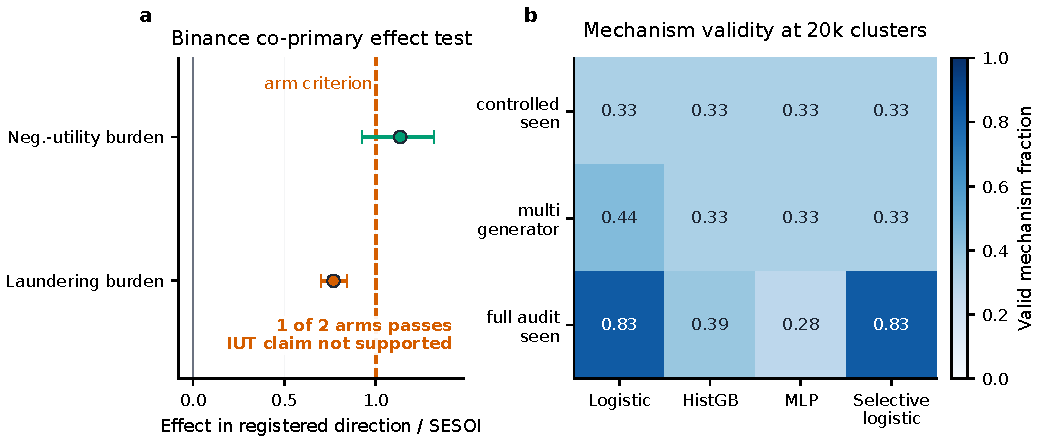
\includegraphics[width=\textwidth]{figures/fig_validity_gates.pdf}
  \Description{Two-panel validity-gate figure. The left panel shows two normalized co-primary effects from the powered Binance order-book test: negative-utility burden exceeds its registered effect threshold, while laundering burden remains below its threshold, so the intersection-union claim fails. The right panel shows valid-mechanism fractions at twenty thousand training clusters for three curricula and four learners.}
  \caption{\textbf{Validity gates preserve partial and undefined evidence.} Panel (a) divides registered Binance effects by their SESOIs; error bars are 95\% cluster-bootstrap intervals and the dashed line is the arm criterion. Planning power uses frozen v0.2 variance. Only one arm passes. Panel (b) reports the fraction of six mechanisms with coverage LCB at least 0.05 at 20,000 clusters; no cell reaches one.}
  \label{fig:validity_gates}
\end{figure*}

\begin{table}[t]
  \caption{Mechanism coverage invalidates most training endpoints (validation only). D0 is outside the data-utility Holm family; the role-neutral control is a negative control.}
  \label{tab:training_validity_supp}
  \centering
  \benchmarktableformat
  % Generated by finauth_audit/paper/generate_tables.py. Do not edit manually.
\begin{tabular}{lrp{0.39\linewidth}}
\toprule
Variant & Valid endpoints & Interpretation \\
\midrule
D0 & 5/5 & prediction diagnostic \\
D1 & 0/5 & authorization reference \\
D2 & 0/5 & authorization variant \\
D3 & 0/5 & authorization variant \\
D4 & 0/5 & authorization variant \\
D5 & 1/5 & authorization variant \\
D6 & 0/5 & authorization variant \\
D7 & 0/5 & authorization variant \\
D7 role-neutral & 0/5 & negative control; outside Holm \\
\bottomrule
\end{tabular}

\end{table}

\begin{table}[t]
  \caption{Holm-adjusted D2--D7 versus D1 validation contrasts. Delta NUAR is \textit{N/A} because no candidate/reference pair has valid endpoints in the same seed.}
  \label{tab:training_holm}
  \centering
  \benchmarktableformat
  % Generated by finauth_audit/paper/generate_tables.py. Do not edit manually.
\begin{tabular}{lrrrrl}
\toprule
Contrast & Delta NUAR & Valid pairs & Raw p & Holm p & Reject \\
\midrule
D2 vs D1 & \textit{N/A} & 0 & 1.000 & 1.000 & no \\
D3 vs D1 & \textit{N/A} & 0 & 1.000 & 1.000 & no \\
D4 vs D1 & \textit{N/A} & 0 & 1.000 & 1.000 & no \\
D5 vs D1 & \textit{N/A} & 0 & 1.000 & 1.000 & no \\
D6 vs D1 & \textit{N/A} & 0 & 1.000 & 1.000 & no \\
D7 vs D1 & \textit{N/A} & 0 & 1.000 & 1.000 & no \\
\bottomrule
\end{tabular}

\end{table}

The D7 role-neutral control masks role and lineage fields during training, calibration, and evaluation. It has 0/5 valid endpoints. Feature-group masking also shows that the fixed learner depends materially on role features: masking them raises D7 validation-unseen NUAR to 0.167 and ALR to 0.165. These are shortcut diagnostics, not causal feature attributions.

The prospective v0.3 robustness study uses Logistic Regression, histogram gradient boosting, MLP, and coverage-constrained selective Logistic; budgets of 400, 1,000, 5,000, and 20,000 independent clusters; controlled-seen, multi-generator, and full-audit-seen curricula; and three frozen seeds. At 20,000 clusters, full-audit Logistic and selective Logistic reach mean valid-mechanism fraction 0.833, but neither has all six mechanisms valid in any seed. Sequential-market validation remains below the fixed 0.05 coverage floor, so complete primary NUAR remains \textit{N/A}. This distinguishes partial endpoint recovery from a valid cross-mechanism comparison.

\section{Paper-Test Stability and Generator Sensitivity}
The paper split reproduces validation rankings, while the prospective mechanisms test whether that stability extends beyond one generator family.

\begin{table}[t]
  \caption{Validation-to-paper and cross-generator rank stability. Constant certification ranks remain \textit{N/A} and are not shown.}
  \label{tab:scale_stability}
  \centering
  \benchmarktableformat
  % Generated by finauth_audit/paper/generate_tables.py. Do not edit manually.
\begin{tabular}{p{0.48\linewidth}p{0.24\linewidth}r}
\toprule
Comparison & Rank & Spearman \\
\midrule
Validation vs paper test & raw FAR & 1.000 \\
Validation vs paper test & certification & 1.000 \\
Institutional vs Sequential & raw FAR & 0.994 \\
Institutional vs Utility IID & raw FAR & 0.738 \\
Sequential vs Utility IID & raw FAR & 0.683 \\
\bottomrule
\end{tabular}

\end{table}

Sequential and institutional generators have raw NUAR-rank Spearman 0.994; their correlations with utility IID are 0.683 and 0.738. Lowest-NUAR and highest-certification rules differ in two of three families. The controlled generators cannot establish a universal financial relationship; they supply interpretable, mechanistically distinct scenarios for auditing rule-by-generator interactions.

\section{Review Workload and Baseline Governance}
Review routing is not a free abstention channel. On validation, Lifecycle Checklist sends 43.5\% of controlled rows to review and exceeds a 40\% review-capacity scenario by 1,383 rows. Of those reviewed cases, 79.7\% would be harmful under direct execution, but only 1.9\% contain a safe positive opportunity. The paper-test review rate is 42.9\%. These are simulated workloads and normalized cost sensitivities, not measured staffing time or reviewer accuracy.

The baseline-governance audit reproduces the registered Lifecycle rule exactly, then evaluates frozen component removals and independently motivated compositions. Role + Confidence + Cost Gate and Lifecycle without the reduce route both achieve validation certification volume 0.60, above the registered Lifecycle value 0.30. Continuous conservative hypervolume instead ranks Hard Role Gate above Lifecycle. These results reject a Lifecycle-only winner narrative and support frontier reporting.

\section{Baseline Field Access}
Deployable rules may use candidate action, confidence, uncertainty, expected edge, cost and liquidity proxies, horizon, current source role, and legal lineage fields declared for their task. They may not use realized returns, post-cost utility, harm labels, oracle opportunity, laundering truth, tail loss, future decoys, or test outcomes. Oracle-positive opportunity and attack labels are evaluation-only. Public rationales, profiles, and user identities are not execution evidence.

The equal-information EPV Adapter uses the same legal fields as other baselines. It is included to test whether low NUAR transfers to provenance safety, not to establish or refute the companion method paper. The overlap audit snapshots the current AAAI source and checks seeds, exact data hashes, exact/perceptual figure hashes, headline claims, and shared 8/12-grams. The current audit reports zero conflicts across those gates; a fresh snapshot is required before submission.

\section{Negative Results and Change Policy}
FinAuth-Audit keeps development failures as audit evidence. The first controlled generator allowed non-opportunity noise to create unintended positive opportunities; a rule-independent correction repaired the density control. The first training endpoint averaged mechanisms before checking per-mechanism coverage and produced a misleading low-NUAR result; the registered endpoint now requires every mechanism to pass its coverage floor. Strict verification later found a cross-layer holdout leak in D4/D5/D7, after which both controlled and provenance holdout families were applied and the affected corpora rebuilt. No test outcome was opened during these changes.

After validation development, the existing test clusters were partitioned using event IDs only. A validation rehearsal reproduced registered outputs, the scientific surface was frozen in a content-addressed archive, and the paper-test evaluator was executed once. After inspection, generator distributions, attack definitions, seeds, feature manifests, certification thresholds, primary endpoints, and robustness profiles cannot change to obtain a preferred ranking. A correction requires a reproducible defect and a versioned record that preserves the original result. The 5,000-cluster community-hidden set remains unevaluated.

\section{Ethics and Responsible Use}
Controlled rows are synthetic authorization scenarios and can encode modeling assumptions or omit institutional constraints. Public rows contain event-market observations, not recommendations. The artifact must not be used to justify live trading, automated approval, or removal of human oversight. Users should report source provenance, decision-time legality, coverage, review load, and structural \textit{N/A}; publishing NUAR alone is insufficient. Any institutional extension should add expert review, privacy controls, jurisdiction-specific policy, and post-launch monitoring before operational use.

\FloatBarrier
